\documentclass{article}


\usepackage{arxiv}

\usepackage[utf8]{inputenc} % allow utf-8 input
\usepackage[T1]{fontenc}    % use 8-bit T1 fonts
\usepackage{hyperref}       % hyperlinks
\usepackage{url}            % simple URL typesetting
\usepackage{booktabs}       % professional-quality tables
\usepackage{amsfonts}       % blackboard math symbols
\usepackage{nicefrac}       % compact symbols for 1/2, etc.
\usepackage{microtype}      % microtypography
\usepackage{lipsum}
\usepackage{comment}

\usepackage{caption}
\usepackage{subcaption}

\usepackage{graphicx}
\graphicspath{ {./images/} }
\usepackage{svg}

\title{Udacity Capstone Project Report \\ Elo Merchant Category Recommendation}

\author{
    Sebastian Mack\\
    Machine Learning Nanodegree\\
    Udacity\\
    \texttt{mack.seb@gmail.com} \\
}

\begin{document}
\maketitle

\newpage

\tableofcontents
\newpage

\listoffigures
\newpage

\section{Definition}
%(approx. 1-2 pages)

\subsection{Project Overview}
% In this section, look to provide a high-level overview of the project in layman’s terms. Questions to ask yourself when writing this section:

% Has an overview of the project been provided, such as the problem domain, project origin, and related datasets or input data?
% Has enough background information been given so that an uninformed reader would understand the problem domain and following problem statement?


As the field of study I selected an interesting topic from the finance industry that caught my attention when a new competition on the data science platform Kaggle had been announced. The initiator of this contest is one of the largest payment brands in Brazil called Elo (refer to \url{https://www.cartaoelo.com.br}) which has built partnerships with merchants in order to offer promotions or discounts to cardholders. Main objective of this project is to understand customer loyalty of the anonymized data that Elo is providing. 

For this project the publicly available data for the "Elo Merchant Category Recommendation" Kaggle competition will be considered. It consists out of the following files:

(\url{https://www.kaggle.com/c/elo-merchant-category-recommendation/data})

\begin{itemize}
\item \textbf{train.csv} - the training set
\item \textbf{test.csv} - the test set 
\item \textbf{sample\_submission.csv} - a sample submission file in the correct format - contains all card\_ids you are expected to predict for
\item \textbf{historical\_transactions.csv} - up to 3 months' worth of historical transactions for each card\_id
\item \textbf{merchants.csv} - additional information about all merchants / merchant\_ids in the dataset
\item \textbf{new\_merchant\_transactions.csv} - two months' worth of data for each card\_id containing all purchases that card\_id made at merchant\_ids that were not visited in the historical data.
\end{itemize}

In addition data field descriptions are provided in \textbf{Data\_Dictionary.xlsx}.

Typically companies work with databases involving structured datasets which is also the case for our domain. There has been a lot of research and development in order to find algorithms and models for such type of data. In recent years especially a technique called stacking is becoming more popular and is achieving state of the art results within the field. For more information refer to \cite{stacked,regression, super, scale}

For me personally this problem is very interesting because it represents a real life problem that not only Elo but many other companies are facing right now. In this situation companies are already acquiring and collecting data with their existing services but still struggle to create a business value out of it. In this particular case we can see that by developing a model that can uncover the signal in customer loyalty, a new business value can be proposed. Both the consumer and the merchants could benefit from a well personalized experience. Furthermore the offering company could gain new clients with this value adding service.



\subsection{Problem Statement}
% In this section, you will want to clearly define the problem that you are trying to solve, including the strategy (outline of tasks) you will use to achieve the desired solution. You should also thoroughly discuss what the intended solution will be for this problem. Questions to ask yourself when writing this section:

% Is the problem statement clearly defined? Will the reader understand what you are expecting to solve?
% Have you thoroughly discussed how you will attempt to solve the problem?
% Is an anticipated solution clearly defined? Will the reader understand what results you are looking for?


The problem that is to be solved can be described as a supervised machine learning problem because the model will be trained based on a given target feature. Since this target variable has a continuous value it can be further classified as a regression problem. A problem of this type can be solved and modeled with various approaches but in this study the most promising will be applied.

The main problem will be to build a model from the given data that can predict a loyalty score for each card\_id given in the test data. Therefor the training data contains several features for each card\_id and separate data files with additional information considering transactions of the card as well as information describing the respective merchants of the purchases.

In order to find a solution to the problem, I will use models and algorithms from supervised machine learning because in our training set we are already given our target variable in form of the loyalty score of each card owner. The specific technique which will be applied to get a model for this project is called stacking. The underlying idea behind stacked generalization was first introduced by a paper \cite{stacked} from Wolpert. In other research \cite{super} it was shown that super learning approaches provide both a fundamental theoretical as well as practical improvement to the construction of a predictor. 

The principals of stacking have not only been proven their potential in acadamic world but also in real applications. In many of the recent kaggle competitions that involved structured data sets the winning models included stacking approaches.

Finally, I will outline the most important steps within my theorectical workflow in order to find a solution for the described problem. A structured approach will be helpful for a reasonable result and to have a scientific discussion on the final model. My planned workflow includes the following steps:

\begin{enumerate}
    \item \textbf{Exploratory Data Analysis (EDA)}: As a first step I will explore the provided data and make an analysis. This includes summarizing properties and visualizing important outcomes. It will be also very useful to identify features that are relevant for the model and also to give hints for transformations that are required for fitting the data.
    \item \textbf{Feature Engineering}: Within this step the knowledge gained from the previous step will be applied to clean the data set and to select important features as well as to define new ones.
    \item \textbf{Train Baseline Model}: When the previous step is completed, the obtained transformed and extended dataset can be used to train the baseline model (or benchmarking model). It will be an implementation of an Ensemble model with gradient boosting for regression.
    \item \textbf{Train Stacked Model}: The most important step is to train our stacked model which will be combined from several weak learners that still have to be selected.
    \item \textbf{Tune paramters}: Since there are lots of parameters available in order to train a suffisticated model, it will be necessary to repeat some of the steps and fine tune the model until it is able to produce the desired scores.
    \item \textbf{Evaluate Metrics}: In the last step, the results and scores of all generated models will be evaluated and compared to one another.

    
\end{enumerate}

In case I am able to build a model with promising outcomes on the testing data, I will also make a submission file for the kaggle competition to get a score for the public leaderboard to test wether my model can compete with the ones from other kagglers.

\subsection{Metrics}
% In this section, you will need to clearly define the metrics or calculations you will use to measure performance of a model or result in your project. These calculations and metrics should be justified based on the characteristics of the problem and problem domain. Questions to ask yourself when writing this section:

% Are the metrics you’ve chosen to measure the performance of your models clearly discussed and defined?
% Have you provided reasonable justification for the metrics chosen based on the problem and solution?


Since one objective of this project is also to produce a submission file for the ongoing kaggle competition, the choosen evaluation metric will be the Root Mean Squared Error (RMSE) as suggested by the rules.

\begin{equation} \label{rmse}
    RMSE = \sqrt{\frac{1}{n}\sum_{i=1}^{n}(y_i-\hat{y_i})^2}
\end{equation}

In our case we can calculate a score with equation (\ref{rmse}) where $\hat{y}$ is the predicted loyalty score for each \texttt{card\_id}, and $y$ is the actual loyalty score assigned to a \texttt{card\_id}.

\newpage
\section{Analysis}
%(approx. 2-4 pages)
Before we begin to model the given problem, an analysis of the given data sets needs to be performed in order to understand which algorithms are going to be used in the next steps of the project. This chapter includes a data exploration which describes characteristic properties of the data as well as visualizations that help to summarize the most important outcomes. In another section of this chapter we discuss different algorithms  that we intend to use for solving the problem given the specific domain. Finally, we  provide a clearly defined benchmark result for comparing across performances obtained by our solution.

\subsection{Data Exploration}
% In this section, you will be expected to analyze the data you are using for the problem. This data can either be in the form of a dataset (or datasets), input data (or input files), or even an environment. The type of data should be thoroughly described and, if possible, have basic statistics and information presented (such as discussion of input features or defining characteristics about the input or environment). Any abnormalities or interesting qualities about the data that may need to be addressed have been identified (such as features that need to be transformed or the possibility of outliers). Questions to ask yourself when writing this section:

% If a dataset is present for this problem, have you thoroughly discussed certain features about the dataset? Has a data sample been provided to the reader?
% If a dataset is present for this problem, are statistics about the dataset calculated and reported? Have any relevant results from this calculation been discussed?
% If a dataset is not present for this problem, has discussion been made about the input space or input data for your problem?
% Are there any abnormalities or characteristics about the input space or dataset that need to be addressed? (categorical variables, missing values, outliers, etc.)

Within this section, we present basic statistics and information that can be extracted from the provided data sets. As can be seen in figure \ref{fig:train_head} which represents the first entries of the training data, it consists out of 6 distinct columns. We can find a column with 201917 unique card ids for each entry as well as a date column with the first active month of the respective card. In addition we are given 3 columns with features (1,2 and 3) that contain categorical values and also the target variable namely the loyalty score of the entry.

\begin{figure}[h]
  \centering
  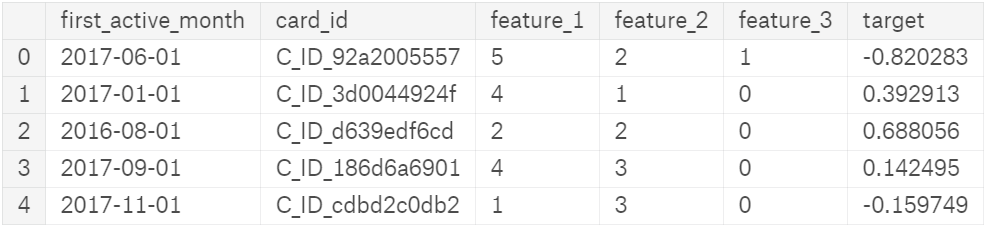
\includegraphics[width=300pt]{train_head}
  \caption{Head of the training data}
  \label{fig:train_head}
\end{figure}

The target variable is a continuous value that ranges in the data set from a minimum value of -33.219281 to a maximum value of 17.965068. In figure \ref{fig:distplot_target} the probability density plot of the loyalty score is shown. We can see that the mean of the target variable is near 0 (-0.393636) and the calculated standard deviation equals 3.850500. It is important to note that the distribution is highly skewed or asymmetric (-6.72016) and has a positive kurtosis (55.031783).

\begin{figure}[h]
  \centering
  \includesvg[width=300pt]{distplot_target}
  \caption{Distribution of the target variable (Loyalty score)}
  \label{fig:distplot_target}
\end{figure}

One observation that can be made from the boxplot (see figure \ref{fig:boxplot_target}) of the loyalty score is that there are many values that can be considered outliers. Although these points do not fall in 1.5 of the IQR we cannot simply remove them because they represent highly loyal or disloyal card owners and are especially from interest in our model.
\newpage

\begin{figure}[h]
  \centering
  \includesvg[width=250pt]{boxplot_target}
  \caption{Boxplot of the target variable (Loyalty score)}
  \label{fig:boxplot_target}
\end{figure}

The test data set contains exactly the same columns as the as the train data set except the target variable which is hidden for the leader board evaluation of the Kaggle competition. It includes 123623 entries with a similar relative distribution (value count) of categories compared to the training data.

Beside the train and test data sets we have additional information about the transactions of each card and about all merchants in different files but since this data needs to be aggregated and combined with the original sets we will discuss it in section \ref{sec:data_preprocessing}. 

\subsection{Exploratory Visualization}
% In this section, you will need to provide some form of visualization that summarizes or extracts a relevant characteristic or feature about the data. The visualization should adequately support the data being used. Discuss why this visualization was chosen and how it is relevant. Questions to ask yourself when writing this section:

% Have you visualized a relevant characteristic or feature about the dataset or input data?
% Is the visualization thoroughly analyzed and discussed?
% If a plot is provided, are the axes, title, and datum clearly defined?

This section provides visualizations that extract the most relevant characteristics about the data. All of the four features to analyze (\texttt{first\_active\_month}, \texttt{feature\_1}, \texttt{feature\_2} and \texttt{feature\_3}) contain categorical values. In figure \ref{fig:catplot_first_active_month} we have a range of the first active month of the card from November 2011 to February 2018. On Exception is the month of January 2011 where no data points can be found in our set. A trend which can be observed in this figure is the increasing amount of active cards in the given time period.

\begin{figure}[h]
  \centering
  \includesvg[width=500pt]{catplot_first_active_month}
  \caption{Plot of value count for each unique category}
  \label{fig:catplot_first_active_month}
\end{figure}

\newpage
\begin{figure}[h]
     \centering
     \begin{subfigure}[b]{0.4\textwidth}
         \centering
         \includesvg[width=\textwidth]{catplot_feature_1}
     \end{subfigure}
     \hfill
     \begin{subfigure}[b]{0.25\textwidth}
         \centering
         \includesvg[width=\textwidth]{catplot_feature_2}
     \end{subfigure}
     \hfill
     \begin{subfigure}[b]{0.2\textwidth}
         \centering
         \includesvg[width=\textwidth]{catplot_feature_3}
     \end{subfigure}
     
    \caption{Plot of value count for each unique category: \texttt{feature\_1}, \texttt{feature\_2} and \texttt{feature\_3}}
    \label{fig:catplot_features}
\end{figure}

As we can see from figure \ref{fig:catplot_features} we have five different categories for \texttt{feature\_1}, three for \texttt{feature\_2} and two for \texttt{feature\_3}. The value counts for each of the categories demonstrate that some of them are more dominant in the data set than others. Within figure \ref{fig:violin_plot_features} the distribution of the target variable (loyalty score) is plotted for each category in form of violin plots. Across all features we can see that the distributions are comparable to one another and all of them have their peaks near 0. 

\begin{figure}[h]
     \centering
     \begin{subfigure}[b]{1\textwidth}
         \centering
         \includesvg[height=150pt]{violin_feature_1}
     \end{subfigure}
     \hfill
     \begin{subfigure}[b]{0.4\textwidth}
         \centering
         \includesvg[height=150pt]{violin_feature_2}
     \end{subfigure}
     \hfill
     \begin{subfigure}[b]{0.5\textwidth}
         \centering
         \includesvg[height=150pt]{violin_feature_3}
     \end{subfigure}
     
    \caption{Violin plot for each unique category of target: \texttt{feature\_1}, \texttt{feature\_2} and \texttt{feature\_3}}
    \label{fig:violin_plot_features}
\end{figure}

For more visualizations please refer to the appendix (\ref{sec:appendix}) which includes several plots of the testing data set and a detailed violin plot of the \texttt{first\_active\_month} feature.

\newpage

\subsection{Algorithms and Techniques}
% In this section, you will need to discuss the algorithms and techniques you intend to use for solving the problem. You should justify the use of each one based on the characteristics of the problem and the problem domain. Questions to ask yourself when writing this section:

% Are the algorithms you will use, including any default variables/parameters in the project clearly defined?
% Are the techniques to be used thoroughly discussed and justified?
% Is it made clear how the input data or datasets will be handled by the algorithms and techniques chosen?

The technique that is being applied in order to solve the given problem is called \textit{Stacking} or \textit{Super Learning}. As it is decribed in \cite{h2o}, ensemble machine learning methods use multiple learning algorithms to obtain better predictive performance than could be obtained from any of the constituent learning algorithms. Many of the popular modern machine learning algorithms are actually ensembles. For example, Random Forest and Gradient Boosting Machine (GBM) are both ensemble learners. Both bagging (e.g. Random Forest) and boosting (e.g. GBM) are methods for ensembling that take a collection of weak learners (e.g. decision tree) and form a single, strong learner.

Stacking is a class of algorithms that involves training a second-level "metalearner" to find the optimal combination of the base learners. Unlike bagging and boosting, the goal in stacking is to ensemble strong, diverse sets of learners together.

For the implementation of this technique we use the \texttt{H20} machine learning framework that provides an supervised ensemble machine learning algorithm for stacking. This Super Learner Algorithm includes the following steps for building a model:

\begin{enumerate}
    \item Set up the ensemble
    \begin{enumerate}
        \item Specify a list of L base algorithms (with a specific set of model parameters)
        \item Specify a metalearning algorithm
    \end{enumerate}
    \item Train the ensemble
    \begin{enumerate}
        \item Train each of the L base algorithms on the training set
        \item Perform k-fold cross-validation on each of these learners and collect the cross-validated predicted values from each of the L algorithms
        \item The N cross-validated predicted values from each of the L algorithms can be combined to form a new N x L matrix. This matrix, along wtih the original response vector, is called the “level-one” data. (N = number of rows in the training set.)
        \item Train the metalearning algorithm on the level-one data. The “ensemble model” consists of the L base learning models and the metalearning model, which can then be used to generate predictions on a test set
    \end{enumerate}
    \item Predict on new data
    \begin{enumerate}
        \item To generate ensemble predictions, first generate predictions from the base learners
        \item Feed those predictions into the metalearner to generate the ensemble prediction
    \end{enumerate}
\end{enumerate}



\subsection{Benchmark}
% In this section, you will need to provide a clearly defined benchmark result or threshold for comparing across performances obtained by your solution. The reasoning behind the benchmark (in the case where it is not an established result) should be discussed. Questions to ask yourself when writing this section:

% Has some result or value been provided that acts as a benchmark for measuring performance?
% Is it clear how this result or value was obtained (whether by data or by hypothesis)?

For benchmarking purposes it was decided to use a Gradient Boosting Machine (GBM) algorithm as bench-marking model which can be compared to the main (stacked) model. The implementation we use is provided by the \texttt{H20} machine learning framework. As it is described in \cite{h2ogbm}, Gradient Boosting Machine for Regression is a forward learning ensemble method.

\begin{table}[h]
 \caption{Results for Cross Validation with a Gradient Boosting Machine (GBM) Benchmark}
  \centering
  \begin{tabular}{lllllllll}
    \toprule
     &          mean & sd & cv\_1 & cv\_2 & cv\_3 & cv\_4 & cv\_5 & cv\_6\\
    \midrule
    mae&        1.6049318&0.0098847&1.6034063&1.6325411&1.6202565&1.6075463&1.6059594&1.5916957\\
    mrd&        14.758833&0.2759703&14.457203&15.389267&15.149721&15.039012&14.56817&14.3106165\\
    mse&        14.758833&0.2759703&14.457203&15.389267&15.149721&15.039012&14.56817&14.3106165\\
    r2&         0.0044686&0.0004175&0.0037364&0.0044269&0.0051961&0.0053651&0.0044451&0.0046830\\
    rd&         14.758833&0.2759703&14.457203&15.389267&15.149721&15.039012&14.56817&14.3106165\\
    rmse&       3.8413863&0.0359411&3.802263&3.9229157&3.8922644&3.8780165&3.816827&3.7829375\\

    \bottomrule
  \end{tabular}
  \label{tab:gbm_results}
\end{table}

\begin{itemize}
    \item Benchmark score on test data (public Kaggle leaderboard): \textbf{3.921}
\end{itemize}

The benchmark model is trained with default parameters without any tuning of hyperparamters. As data input the training data from the competition is used without any feature engineering beside the transformation of dates and data types.

\newpage
\section{Methodology}
%(approx. 3-5 pages)
In this chapter we discuss the methodology that has been applied to the given problem. It includes the steps for prepocessing the data in order to address any abnormalities or characteristics. Furthermore, it documents the implemented metrics, algorithms and techniques.

\subsection{Data Preprocessing}
\label{sec:data_preprocessing}
% In this section, all of your preprocessing steps will need to be clearly documented, if any were necessary. From the previous section, any of the abnormalities or characteristics that you identified about the dataset will be addressed and corrected here. Questions to ask yourself when writing this section:

% If the algorithms chosen require preprocessing steps like feature selection or feature transformations, have they been properly documented?
% Based on the Data Exploration section, if there were abnormalities or characteristics that needed to be addressed, have they been properly corrected?
% If no preprocessing is needed, has it been made clear why?

The first thing to notice about the given data is that it is very clean presumably because it has already been extensively preprocessed by the competition host. In the training and testing data we have zero missing values and the additional data sets for transactions and merchants contain only a small fraction (below 0.1 \%) which will be handled depending on the respective feature.

After loading the data sets, an important step is to define the data type for each column, because the framework pandas for structured data can handle it more efficiently. This has especially advantages for the usage of memory because data types like \texttt{float} allocate more space in memory than for example simple \texttt{int} or \texttt{bool}. In our situation, a clever assignment of data types resulted in memory savings up to several Gb of the RAM.

Feature engineering for this domain can be seen as probably the most important part to gain good results. A few basic features could be added to the training and testing data frames without aggregating data from additional sources. The following features have been created directly:


\begin{table}[h]
 \caption{New direct features for Train and Test data sets}
  \centering
  \begin{tabular}{ll}
    \toprule
    Feature & Description\\
    \midrule
    year & Year derived from the first\_active\_month feature\\
    weekofyear & Week as integer derived from the first\_active\_month feature\\
    month & Month as integer derived from the first\_active\_month feature\\
    elapsed\_time & Time difference in days between reference date and first\_active\_month date\\
    \bottomrule
  \end{tabular}
  \label{tab:table_train_test}
\end{table}

In addition several other features have been aggregated from the \texttt{historical\_transactions} and \texttt{new\_merchant\_transactions} data sources. A cleanup that was necessary for both files, is to map the given strings "Y" and "N" to binary values (1 and 0) in the "category\_1" and "authorized\_flag" columns. For the "category\_2" column we used a lambda function to reduce strings (e.g. 1.00000) to their shorter integer format (1) without loosing any information.

The feature "purchase\_date" can be used to create other features and in contrast to the date from the train and test data sets, the purchase dates also includes the time of the purchase. For this reason we can derive the features shown in table \ref{tab:table_hist_new}.

\begin{table}[h]
 \caption{New features for historical transactions and new merchant transactions}
  \centering
  \begin{tabular}{ll}
    \toprule
    Feature & Description\\
    \midrule
    purchase\_year & Year as integer derived from the purchase\_date feature\\
    purchase\_month & Month as integer derived from the purchase\_date feature\\
    purchase\_weekofyear & Week of year as integer derived from the purchase\_date feature\\
    purchase\_dayofweek & Day of week as integer derived from the purchase\_date feature\\
    purchase\_hour & Hour as integer derived from the purchase\_date feature\\
    purchase\_date & Date transformed to int64 * 1e-9\\
    month\_diff & Time difference in days between reference date and purchase\_date date\\
    \bottomrule
  \end{tabular}
  \label{tab:table_hist_new}
\end{table}

In the given data sets for historical transactions and new merchant transactions several transactions can be found for each unique card\_id (owner). Since our target variable is the loyalty score for each card owner in the train and test data, it is not simply possible to merge all of the transaction data into those frames.

\newpage

\begin{table}[h]
 \caption{Aggregated features for Train and Test data sets}
  \centering
  \begin{tabular}{ll}
    \toprule
    Feature & Aggregation Function\\
    \midrule
    purchase\_amount, installments & sum, max, min, mean, var\\
    purchase\_date & max , min\\
    month\_lag, purchase\_month & max, min, mean, var\\
    month\_diff & mean\\
    card\_id & size\\
    category (all 9), authorized\_flag & sum, mean\\
    purchase\_year, purchase\_weekofyear, \\
    purchase\_dayofweek,  purchase\_hour,  subsector\_id,\\
    merchant\_id, merchant\_category\_id & nunique \\
    \bottomrule
  \end{tabular}
  \label{tab:table_agg}
\end{table}

For the aggregation of features for each card id several functions are defined in table \ref{tab:table_agg} and a complete list of features can be found in the appendix. Both the aggegated historical transaction features and the new merchant transactions are merged on the respective card id. Furthermore it is to mention that aggregation and merging had to be performed for each dataframe separately because otherwise we ran into memory issues.


\subsection{Implementation}
% In this section, the process for which metrics, algorithms, and techniques that you implemented for the given data will need to be clearly documented. It should be abundantly clear how the implementation was carried out, and discussion should be made regarding any complications that occurred during this process. Questions to ask yourself when writing this section:

% Is it made clear how the algorithms and techniques were implemented with the given datasets or input data?
% Were there any complications with the original metrics or techniques that required changing prior to acquiring a solution?
% Was there any part of the coding process (e.g., writing complicated functions) that should be documented?

In the previous section, we described the engineering of features and construction of the input data of the model in form of train and test data sets. This input is used in the definition of our model architecture which will make use of Stacking. 

As described in \cite{h2olevel} the architecture makes use of two different types of data as it can be seen in the figures below. The so called "Level Zero" data (the input data) is used by the base learners. One the higher level we combine the predictions of the base learners into a new "Level One" data frame which is used by the super learner.

The following steps have been performed in the implementation phase:
\begin{enumerate}
    \item Define matrix, X (input data: train and test), and response, y (target: loyalty score)
    \item Specify L base learners (with model params)
    \item Specify a metalearner
    \item Perform k-fold CV on each of the L learners
\end{enumerate}

\begin{figure}[h]
  \centering
  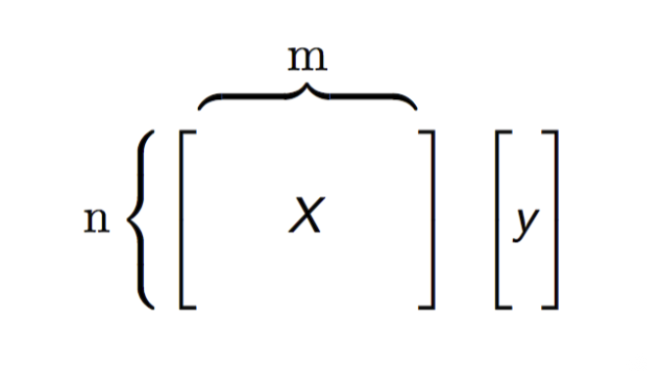
\includegraphics[width=100pt]{level_zero_data}
  \caption{"Level Zero" data}
  \label{fig:level_zero_data}
\end{figure}

\begin{enumerate}
    \item Collect the predicted values from k-fold CV that was
performed on each of the L base learners
    \item Column-bind these prediction vectors together to
form a new design matrix, Z
    \item Train the metalearner using Z, y
\end{enumerate}


\begin{figure}[h]
  \centering
  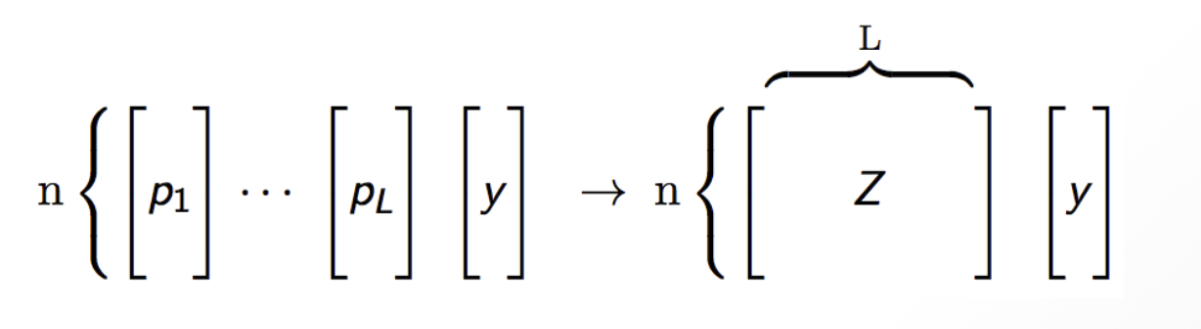
\includegraphics[width=200pt]{level_one_data}
  \caption{"Level One" data}
  \label{fig:level_one_data}
\end{figure}

\newpage
For practical implementation purposes we use the following frameworks:

\begin{itemize}
    \item H2OGradientBoostingEstimator (h2o.estimators.gbm)
    \item H2OGeneralizedLinearEstimator (h2o.estimators.glm)
    \item H2ORandomForestEstimator (h2o.estimators.random\_forest)
    \item H2OStackedEnsembleEstimator (h2o.estimators.stackedensemble)
    \item numpy
    \item pandas
    \item matplotlib, seaborn
\end{itemize}

It is very important to notice that all base models must have the same cross-validation folds and the cross-validated predicted values must be kept because the H2OStackedEnsembleEstimator will use them to form the "Level One" data.


\subsection{Refinement}
% In this section, you will need to discuss the process of improvement you made upon the algorithms and techniques you used in your implementation. For example, adjusting parameters for certain models to acquire improved solutions would fall under the refinement category. Your initial and final solutions should be reported, as well as any significant intermediate results as necessary. Questions to ask yourself when writing this section:

% Has an initial solution been found and clearly reported?
% Is the process of improvement clearly documented, such as what techniques were used?
% Are intermediate and final solutions clearly reported as the process is improved?

Before training the stacked model we experimented with the benchmark model (H2OGradientBoostingEstimator) in order to tune the parameters in a grid search approach consider the following hyperparameters:

hyper\_params = {\\
"learn\_rate": [0.01, 0.03], \\
- Specifies the learning rate. The range is 0.0 to 1.0\\
"max\_depth": [4, 6, 8, 12, 16, 20], \\
- Specifies the maximum tree depth. Higher values will make the model more complex and can lead to overfitting).\\
"sample\_rate": [0.6, 0.8, 1.0], \\
- Specifies the row sampling rate (x-axis).\\
"col\_sample\_rate": [0.6, 0.8, 1.0]\\
- Specifies the column sampling rate (y-axis).}

This resulted in the in an optimal setup with learn\_rate=0.01, max\_depth=6,  sample\_rate=0.8 and col\_sample\_rate=0.8 which will be used for the gbm estimator in the stacked model. 

\underline{Reported regression model metrics on train data}\\
\textbf{MSE}: 13.187148162028853\\
\textbf{RMSE}: 3.631411318210711\\
\textbf{MAE}: 1.542065760164572\\
\textbf{Mean Residual Deviance}: 13.187148162028853

\underline{Reported regression model metrics on cross-validation data}\\
\textbf{MSE}: 13.602099833569243\\
\textbf{RMSE}: 3.6881024705896177\\
\textbf{MAE}: 1.5562552491244939\\
\textbf{Mean Residual Deviance}: 13.602099833569243

\newpage
\section{Results}
%(approx. 2-3 pages)
In this chapter we present the results of the combined super learning model and evaluate metrics that describe it. As a conclusion we will justify our solution by comparing it to the chosen benchmark model.

\subsection{Model Evaluation and Validation}
% In this section, the final model and any supporting qualities should be evaluated in detail. It should be clear how the final model was derived and why this model was chosen. In addition, some type of analysis should be used to validate the robustness of this model and its solution, such as manipulating the input data or environment to see how the model’s solution is affected (this is called sensitivity analysis). Questions to ask yourself when writing this section:

% Is the final model reasonable and aligning with solution expectations? Are the final parameters of the model appropriate?
% Has the final model been tested with various inputs to evaluate whether the model generalizes well to unseen data?
% Is the model robust enough for the problem? Do small perturbations (changes) in training data or the input space greatly affect the results?
% Can results found from the model be trusted?

In tables \ref{tab:glm_results}, \ref{tab:drf_results} and \ref{tab:gbm_results} we summarized the results from the 3 different Base Learners (GLM, DRF, GBM) by performing kfold cross validation (k=6). The fold assigment has been the same for all of the Base Learners in order to compare them and in addition this is a prerequesite for the stacking process.

By comparing the mean value for the rmse metric of the Base Learners, we can already apply a ranking between them across the cross validation data. Best results have been produced by the GBM (3.673) followed by the DRF (3.726) and GLM (3.830). When we look at the cross validation results among the 6 folds, it can be noticed that the models are robust against pertubations in the training data. We assume that especially the distribution of outliers in the folds could be the responsible for small changes. 

In order to test if the models generalize well to unseen data, each one has also been evaluated against the public Kaggle leaderboard. The ranking among them is unchanged but we obtain slightly worse rmse scores: GBM (3.752) followed by the DRF (3.778) and GLM (3.906).


\begin{table}[h]
 \caption{Results for Cross Validation with a Generalized Linear Model (GLM) Base Learner}
  \centering
  \begin{tabular}{lllllllll}
    \toprule
     &          mean & sd & cv\_1 & cv\_2 & cv\_3 & cv\_4 & cv\_5 & cv\_6\\
    \midrule
    mae&        1.581836&0.0203363&1.5764347&1.5607811&1.6022342&1.628451&1.5383326&1.584782\\
    mrd&        14.688586&0.6209948&14.677058&14.209316&15.113588&16.225391&13.331208&14.574956\\
    mse&        14.688586&0.6209948&14.677058&14.209316&15.113588&16.225391&13.331208&14.574956\\
    r2&         0.0092557&0.0003340&0.0089441&0.0095686&0.0092110&0.0085077&0.0100180&0.0092848\\
    rd&         494312.56&20898.559&493927.03&478186.12&508617.6&546033.06&448635.16&490476.4\\
    rmse&       3.8308656&0.0807933&3.831065&3.7695246&3.88762&4.028075&3.6511927&3.8177161\\
    \bottomrule
  \end{tabular}
  \label{tab:glm_results}
\end{table}

\begin{itemize}
    \item GLM Base Learner score on test data (public Kaggle leaderboard): \textbf{3.906}
\end{itemize}

\begin{table}[h]
 \caption{Results for Cross Validation with a Distributed Random Forest (DRF) Base Learner}
  \centering
  \begin{tabular}{lllllllll}
    \toprule
     &          mean & sd & cv\_1 & cv\_2 & cv\_3 & cv\_4 & cv\_5 & cv\_6\\
    \midrule
    mae&        1.6385423&0.0183705&1.6239307&1.6273823&1.6647147&1.6719296&1.595753&1.6475433\\
    mrd&        13.899682&0.556475&13.843744&13.750434&14.459413&15.067332&12.484625&13.792545\\
    mse&        13.899682&0.556475&13.843744&13.750434&14.459413&15.067332&12.484625&13.792545\\
    r2&         0.0622485&0.0088655&0.0652129&0.0415541&0.0520963&0.0792737&0.0728857&0.0624682\\
    rd&         13.899682&0.556475&13.843744&13.750434&14.459413&15.067332&12.484625&13.792545\\
    rmse&       3.7267144&0.0751078&3.7207184&3.7081578&3.8025534&3.8816662&3.5333588&3.7138317\\
    \bottomrule
  \end{tabular}
  \label{tab:drf_results}
\end{table}

\begin{itemize}
    \item DRF Base Learner score on test data (public Kaggle leaderboard): \textbf{3.778}
\end{itemize}

\begin{table}[h]
 \caption{Results for Cross Validation with a Gradient Boosting Machine (GBM) Base Learner}
  \centering
  \begin{tabular}{lllllllll}
    \toprule
     &          mean & sd & cv\_1 & cv\_2 & cv\_3 & cv\_4 & cv\_5 & cv\_6\\
    \midrule
    mae&        1.5640444&0.0184761&1.5589854&1.5495439&1.5860294&1.6010317&1.5195141&1.5691615\\
    mrd&        13.504545&0.5703331&13.43026&13.37311&14.004401&14.745635&12.061675&13.412193\\
    mse&        13.504545&0.5703331&13.43026&13.37311&14.004401&14.745635&12.061675&13.412193\\
    r2&         0.0890768&0.0084026&0.0931331&0.0678547&0.0819251&0.0989318&0.1042942&0.0883222\\
    rd&         13.504545&0.5703331&13.43026&13.37311&14.004401&14.745635&12.061675&13.412193\\
    rmse&       3.6731944&0.0780653&3.6647317&3.6569262&3.7422454&3.8400044&3.4729922&3.6622663\\
    \bottomrule
  \end{tabular}
  \label{tab:gbm_results}
\end{table}

\begin{itemize}
    \item GBM Base Learner score on test data (public Kaggle leaderboard): \textbf{3.752}
\end{itemize}

The final model is, as mentioned before, a Super (Meta) Learner in form of another GLM model that predicts the target by combining the predictions of the Base Learners. It shows reasonable results and achieves the best metrics for rmse on the training data (refer to table \ref{tab:train_comparison}). Furthermore, we can state that it generalizes well to unseen data with a final rmse of 3.727 on the test data set.

\begin{table}[h]
 \caption{Comparison of results reported on train data}
  \centering
  \begin{tabular}{llllll}
    \toprule
     &          Stacked Model & Benchmark Model & GLM & DRF & GBM \\
    \midrule
    mae&        1.522925&1.603647&1.582077&1.671510&1.541610\\
    mse&        12.019943&14.732459&14.657957&14.256069&12.859487\\
    rmse&       3.466979&3.838288&3.828571&3.775721&3.586012\\
    \bottomrule
  \end{tabular}
  \label{tab:train_comparison}
\end{table}

\begin{itemize}
    \item Super Learner score on test data (public Kaggle leaderboard): \textbf{3.727}
\end{itemize}

\subsection{Justification}
% In this section, your model’s final solution and its results should be compared to the benchmark you established earlier in the project using some type of statistical analysis. You should also justify whether these results and the solution are significant enough to have solved the problem posed in the project. Questions to ask yourself when writing this section:

% Are the final results found stronger than the benchmark result reported earlier?
% Have you thoroughly analyzed and discussed the final solution?
% Is the final solution significant enough to have solved the problem?

The overall results (refer to table \ref{tab:test_comparison}) on the hidden test data of the competition can be seen as a confirmation for the quality of the final stacked model. At the moment of writing this report, we achieved a ranking in the top 50\% of competitors which is a reasonably good result under the assumption that many of the other participants are using stacked approaches as well in order to train their models.

\begin{table}[h]
 \caption{Comparison of results reported on test data (public Kaggle leaderboard)}
  \centering
  \begin{tabular}{llllll}
    \toprule
     &          Stacked Model & Benchmark Model & GLM & DRF & GBM \\
    \midrule
    rmse&       \textbf{3.727}&3.921&3.906&3.778&3.752\\
    \bottomrule
  \end{tabular}
  \label{tab:test_comparison}
\end{table}

One remarkable aspect about the chosen model or architecture can also be seen once again for the testing data. Not only can we outperform our benchmarking model with Super Learning but also all of the other models that were used as Base Models. This supports the groundlying concept that each model for its own has advantages and disadvantages over other models. Basically in the data we could find areas where some model is better than its counterpart but there may be different areas where it is the other way around. For this reason stacked approaches can benefit from the diversity of their base models.


\newpage
\section{Conclusion}
%(approx. 1-2 pages)
Finally, we use this last chapter to summarize the most important outcomes that have been produced by our project. A free-form visualization emphasizes interesting characteristics of the modeling results which are hinting to relevant features for predicting customer loyalty. Furthermore, we reflect on the entire process we used for this project and give a brief outlook for upcoming improvements to the model.

\subsection{Free-Form Visualization}
% In this section, you will need to provide some form of visualization that emphasizes an important quality about the project. It is much more free-form, but should reasonably support a significant result or characteristic about the problem that you want to discuss. Questions to ask yourself when writing this section:

% Have you visualized a relevant or important quality about the problem, dataset, input data, or results?
% Is the visualization thoroughly analyzed and discussed?
% If a plot is provided, are the axes, title, and datum clearly defined?

One of the most interesting parts about models like Gradient Boosted Machines (GBM) is the option to obtain the importance of features or variables from the created model. This is especially helpful in understanding the given problem or data set and also provides an insight how the model predicts the target variable.

\begin{figure}[h]
  \centering
  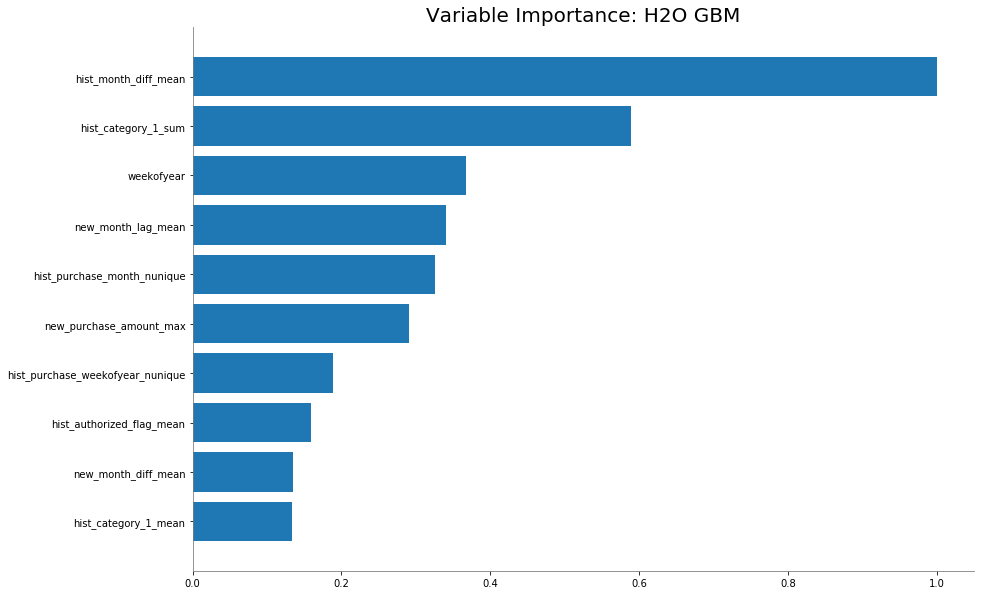
\includegraphics[width=350pt]{gbm_variable_importance}
  \caption{GBM Feature Importance Plot}
  \label{fig:gbm_variable_importance}
\end{figure}

As can be seen in figure \ref{fig:gbm_variable_importance}, many of the 10 most important features are the ones that have been engineered. The feature with the highest scaled importance value is called "hist\_month\_diff\_mean" and represents the mean of temporal differences (reference date - purchase date in months) for aggregated historical transactions of each card id. We can also see that the week of the year ("weekofyear") in which the customer was first active plays a big role in predicting his loyalty. Some of the features also proof some intuitions that could be made about the problem, e.g. that the mean of transactions that have been approved ("hist\_authorized\_flag\_mean") or also the max purchase amount of new transactions ("new\_purchase\_amount\_max") are highly relevant for the target variable. Although we can find categorical variables like "hist\_category\_1\_sum, -mean", it is very interesting that the top 10 of features is dominated by temporal information.

\subsection{Reflection}
% In this section, you will summarize the entire end-to-end problem solution and discuss one or two particular aspects of the project you found interesting or difficult. You are expected to reflect on the project as a whole to show that you have a firm understanding of the entire process employed in your work. Questions to ask yourself when writing this section:

% Have you thoroughly summarized the entire process you used for this project?
% Were there any interesting aspects of the project?
% Were there any difficult aspects of the project?
% Does the final model and solution fit your expectations for the problem, and should it be used in a general setting to solve these types of problems?

The process we followed for this project basically consisted out of the six phases shown in figure \ref{fig:process}. As a first step the problem needed to be defined and described clearly with a given metric for evaluation. Second, we performed an analysis of the given data for the problem and identified its most important characteristics. Also several visualizations are provided to summarize relevant properties. 

Next, many preprocessing steps to clean and transform values have been necessary before we could start to engineer new features for training. Feature engineering was an aspect that has proven to be extraordinary difficult and required a lot of trial and error as well as several days of tuning. In addition, because most of the features in the data had only a generalized naming convention like "feature\_1" or "category\_3" it was hard to understand the background.

Finally, the most interesting part of the project was the modeling phase followed be the evaluation. The idea of stacked ensembles is still fascinating that by combining different base learners into a super learner we can take advantages from all of them and create a more versatile and flexible model that generalizes well to unseen data. It was very pleasant to see that a super learning model approach is not only in scientific theory a good choice but also proves to be extremely effective in real world applications. Although the presented final stacked model could not quite compete in the kaggle leaderboard with the top models, it was demonstrated that it performs still way better than the benchmarking model and base learners.

\begin{figure}[h]
  \centering
  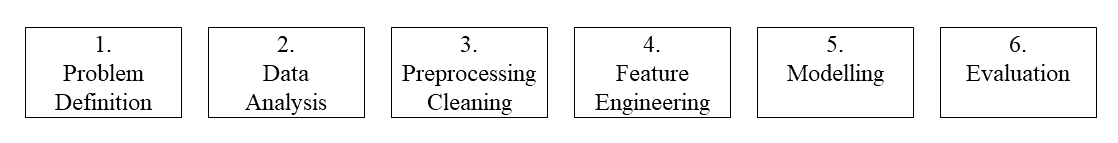
\includegraphics[width=350pt]{process}
  \caption{Project Process}
  \label{fig:process}
\end{figure}

\subsection{Improvement}
% In this section, you will need to provide discussion as to how one aspect of the implementation you designed could be improved. As an example, consider ways your implementation can be made more general, and what would need to be modified. You do not need to make this improvement, but the potential solutions resulting from these changes are considered and compared/contrasted to your current solution. Questions to ask yourself when writing this section:

% Are there further improvements that could be made on the algorithms or techniques you used in this project?
% Were there algorithms or techniques you researched that you did not know how to implement, but would consider using if you knew how?
% If you used your final solution as the new benchmark, do you think an even better solution exists?

As can be seen from the public score of our final model in the Kaggle competition leaderboard, there is still a lot of room for improvements (at the moment top world participants reach RMSE scores around 3.647 and the competition is still ongoing). Although the provided model is able to predict the loyalty score of card owners quite acurately, at least in the following areas of the modeling improvements can be made in the future:

\begin{enumerate}
    \item \textbf{Feature Engineering}: We have seen that especially aggregating new features from the historical transactions and new merchant transaction lead to high differences in the scoring metric. For this reason it would be a good idea to take an even closer look at how to combine and aggregate new features. In addition we have not taken the information about the different merchant ids where to purchase was made into account and could aggregate several other features from this file.
    \item \textbf{Tuning of the Base Learners}: Until now only one of the Base Learner (GBM) could be tuned sufficiently due to time constraints and computational effort. It would make sense to also apply hyperparameter tuning for all of the other remaining Base Learner. An example is to use a randomized grid search approach to fine tune the relevant parameters
    \item \textbf{Selection of the Base Learners}: In order to give our SUper Learner the chance to learn from a wide variety of models we can add more Base Learners to the final model. One candidate that has not been included yet is a Deep Learing Algorithm, since it is very difficult to find a proper architecture and fitting parameters. Furthermore beside only adding a single model for each algorithm, it would also be possible to add multiple models of the same class (grid of models with different paramters). 
    \item \textbf{Tuning of the Super (Meta) Learner}: As before also the Super Learner Parameters can be adjusted and tuned e.g. with a grid search approach.
    \item \textbf{Selection of the Super (Meta) Learner}: In our model we used a Generalized Linear Model for ensembling of the Base Learner, but other models like Gradient Boosting Machines, Random Forest or even Deep Neural Networks are possible. It needs to be investigated if one of these approaches can lead to significantly better results than the present one.
    \item \textbf{Stratified KFold}: In addition to the previous improvements, a training strategy where the cross validation is not performed on random folds but on stratified folds that preserve the percentage of samples for each class. The target variable of our class is not a category but with some tricks we can include in each fold a fair amount of outliers which will be a better representation for testing the kfolded data.

\end{enumerate}

By applying some of these modelling approaches we are pretty confident that the model can be further improved and also a better ranking in the Kaggle leaderboard is reachable.



\newpage
\bibliographystyle{unsrt}
\bibliography{references}

\newpage
\section{Appendix}
\label{sec:appendix}

\subsection{Additional Feature plots for test data}
\begin{figure}[h]
  \centering
  \includesvg[width=500pt]{catplot_first_active_month_test}
  \caption{Plot of value count for each unique category: \texttt{first\_active\_month}}
  \label{fig:catplot_first_active_month_test}
\end{figure}

\begin{figure}[h]
     \centering
     \begin{subfigure}[b]{0.4\textwidth}
         \centering
         \includesvg[width=\textwidth]{catplot_feature_1_test}
     \end{subfigure}
     \hfill
     \begin{subfigure}[b]{0.25\textwidth}
         \centering
         \includesvg[width=\textwidth]{catplot_feature_2_test}
     \end{subfigure}
     \hfill
     \begin{subfigure}[b]{0.2\textwidth}
         \centering
         \includesvg[width=\textwidth]{catplot_feature_3_test}
     \end{subfigure}
        \caption{Plot of value count for each unique category: \texttt{feature\_1}, \texttt{feature\_2} and \texttt{feature\_3}}
        \label{fig:catplot_features_test}
\end{figure}

\newpage
\subsection{Violin plot first active month}

\begin{figure}[h]
  \centering
  \includesvg[width=500pt]{violin_first_active_month}
  \caption{Violin plot for each unique category of target: \texttt{first\_active\_month}}
  \label{fig:violin_first_active_month_test}
\end{figure}

\newpage

\subsection{List of Features}

\begin{enumerate}
\item feature\_1
\item feature\_2
\item feature\_3
\item hist\_purchase\_date\_max
\item hist\_purchase\_date\_min
\item hist\_month\_diff\_mean
\item hist\_card\_id\_size
\item hist\_purchase\_amount\_sum
\item hist\_purchase\_amount\_max
\item hist\_purchase\_amount\_min
\item hist\_purchase\_amount\_mean
\item hist\_purchase\_amount\_var
\item hist\_installments\_sum
\item hist\_installments\_max
\item hist\_installments\_min
\item hist\_installments\_mean
\item hist\_installments\_var
\item hist\_month\_lag\_sum
\item hist\_month\_lag\_max
\item hist\_month\_lag\_min
\item hist\_month\_lag\_mean
\item hist\_month\_lag\_var
\item hist\_authorized\_flag\_sum
\item hist\_authorized\_flag\_mean
\item hist\_purchase\_weekend\_sum
\item hist\_purchase\_weekend\_mean
\item hist\_category\_1\_sum
\item hist\_category\_1\_mean
\item hist\_category\_2\_1\_sum
\item hist\_category\_2\_1\_mean
\item hist\_category\_2\_2\_sum
\item hist\_category\_2\_2\_mean
\item hist\_category\_2\_3\_sum
\item hist\_category\_2\_3\_mean
\item hist\_category\_2\_4\_sum
\item hist\_category\_2\_4\_mean
\item hist\_category\_2\_5\_sum
\item hist\_category\_2\_5\_mean
\item hist\_category\_3\_A\_sum
\item hist\_category\_3\_A\_mean
\item hist\_category\_3\_B\_sum
\item hist\_category\_3\_B\_mean
\item hist\_category\_3\_C\_sum
\item hist\_category\_3\_C\_mean
\item hist\_purchase\_year\_nunique
\item hist\_purchase\_weekofyear\_nunique
\item hist\_purchase\_month\_nunique
\item hist\_purchase\_dayofweek\_nunique
\item hist\_purchase\_hour\_nunique
\item hist\_subsector\_id\_nunique
\item hist\_merchant\_id\_nunique
\item hist\_merchant\_category\_id\_nunique
\item new\_purchase\_date\_max
\item new\_purchase\_date\_min
\item new\_month\_diff\_mean
\item new\_card\_id\_size
\item new\_purchase\_amount\_sum
\item new\_purchase\_amount\_max
\item new\_purchase\_amount\_min
\item new\_purchase\_amount\_mean
\item new\_purchase\_amount\_var
\item new\_installments\_sum
\item new\_installments\_max
\item new\_installments\_min
\item new\_installments\_mean
\item new\_installments\_var
\item new\_month\_lag\_sum
\item new\_month\_lag\_max
\item new\_month\_lag\_min
\item new\_month\_lag\_mean
\item new\_month\_lag\_var
\item new\_authorized\_flag\_sum
\item new\_authorized\_flag\_mean
\item new\_purchase\_weekend\_sum
\item new\_purchase\_weekend\_mean
\item new\_category\_1\_sum
\item new\_category\_1\_mean
\item new\_category\_2\_1\_sum
\item new\_category\_2\_1\_mean
\item new\_category\_2\_2\_sum
\item new\_category\_2\_2\_mean
\item new\_category\_2\_3\_sum
\item new\_category\_2\_3\_mean
\item new\_category\_2\_4\_sum
\item new\_category\_2\_4\_mean
\item new\_category\_2\_5\_sum
\item new\_category\_2\_5\_mean
\item new\_category\_3\_A\_sum
\item new\_category\_3\_A\_mean
\item new\_category\_3\_B\_sum
\item new\_category\_3\_B\_mean
\item new\_category\_3\_C\_sum
\item new\_category\_3\_C\_mean
\item new\_purchase\_year\_nunique
\item new\_purchase\_weekofyear\_nunique
\item new\_purchase\_month\_nunique
\item new\_purchase\_dayofweek\_nunique
\item new\_purchase\_hour\_nunique
\item new\_subsector\_id\_nunique
\item new\_merchant\_id\_nunique
\item new\_merchant\_category\_id\_nunique
\item year
\item weekofyear
\item month
\item elapsed\_time
\item hist\_purchase\_date\_diff
\item hist\_purchase\_date\_average
\item hist\_purchase\_date\_uptonow
\item hist\_first\_buy
\item new\_first\_buy
\item card\_id\_total
\item purchase\_amount\_total
\end{enumerate}

% Before submitting, ask yourself. . .

% Does the project report you’ve written follow a well-organized structure similar to that of the project template?
% Is each section (particularly Analysis and Methodology) written in a clear, concise and specific fashion? Are there any ambiguous terms or phrases that need clarification?
% Would the intended audience of your project be able to understand your analysis, methods, and results?
% Have you properly proof-read your project report to assure there are minimal grammatical and spelling mistakes?
% Are all the resources used for this project correctly cited and referenced?
% Is the code that implements your solution easily readable and properly commented?
% Does the code execute without error and produce results similar to those reported?





















































\begin{comment}

\section{+++++++++++++++++++++++++++++++++++++++++++++++++++++++++++++}

\section{Headings: first level}
\label{sec:headings}

\lipsum[4] See Section \ref{sec:headings}.

\subsection{Headings: second level}
\lipsum[5]
\begin{equation}
\xi _{ij}(t)=P(x_{t}=i,x_{t+1}=j|y,v,w;\theta)= {\frac {\alpha _{i}(t)a^{w_t}_{ij}\beta _{j}(t+1)b^{v_{t+1}}_{j}(y_{t+1})}{\sum _{i=1}^{N} \sum _{j=1}^{N} \alpha _{i}(t)a^{w_t}_{ij}\beta _{j}(t+1)b^{v_{t+1}}_{j}(y_{t+1})}}
\end{equation}

\subsubsection{Headings: third level}
\lipsum[6]

\paragraph{Paragraph}
\lipsum[7]

\section{Examples of citations, figures, tables, references}
\label{sec:others}
\lipsum[8] \cite{kour2014real,kour2014fast} and see \cite{hadash2018estimate}.

The documentation for \verb+natbib+ may be found at
\begin{center}
  \url{http://mirrors.ctan.org/macros/latex/contrib/natbib/natnotes.pdf}
\end{center}
Of note is the command \verb+\citet+, which produces citations
appropriate for use in inline text.  For example,
\begin{verbatim}
   \citet{hasselmo} investigated\dots
\end{verbatim}
produces
\begin{quote}
  Hasselmo, et al.\ (1995) investigated\dots
\end{quote}

\begin{center}
  \url{https://www.ctan.org/pkg/booktabs}
\end{center}


\subsection{Figures}
\lipsum[10] 
See Figure \ref{fig:fig1}. Here is how you add footnotes. \footnote{Sample of the first footnote.}
\lipsum[11] 

\begin{figure}
  \centering
  \includesvg[width=400pt]{fig1}
  \caption{Sample figure caption.}
  \label{fig:distplot}
\end{figure}

\subsection{Tables}
\lipsum[12]
See awesome Table~\ref{tab:table}.

\begin{table}
 \caption{Sample table title}
  \centering
  \begin{tabular}{lll}
    \toprule
    \multicolumn{2}{c}{Part}                   \\
    \cmidrule(r){1-2}
    Name     & Description     & Size ($\mu$m) \\
    \midrule
    Dendrite & Input terminal  & $\sim$100     \\
    Axon     & Output terminal & $\sim$10      \\
    Soma     & Cell body       & up to $10^6$  \\
    \bottomrule
  \end{tabular}
  \label{tab:table}
\end{table}

\subsection{Lists}
\begin{itemize}
\item Lorem ipsum dolor sit amet
\item consectetur adipiscing elit. 
\item Aliquam dignissim blandit est, in dictum tortor gravida eget. In ac rutrum magna.
\end{itemize}
\end{comment}



\end{document}
